\chapter{Word Embedding}
\section{Monolingual Embedding}
	Word embeddings is distributed representation of words in a vector space. With the learning algorithm it can capture the contextual or co-occurrence information. The word embedding has an interesting and important property: similar words will have similar distribution in the embedding space, with that property, we can find meaningful near-synonyms or  Some successful methods for learning word embeddings like word2vec  \cite{mikolov2013distributed}
	Continuous Bag-of-Words model(CBOW) and Skip-Gram model
	CBOW model and Skip-Gram model are currently the  common structures to learn the word embedding. Algorithmically,  CBOW tries to predict the current word based on the context while Skip-Gram model tries to maximize classification of a word based on another word in the same sentence.
	The neural probability language model defines the prediction probability using the softmax function:

	
	\begin{align}
	p(w_t | w_s) & = \textrm{softmax} {(s(w_t, w_s))} \\
	& = \frac{\exp\{s(w_t, w_s)\}}{\sum_{w^{\prime} \in W}{\exp\{s( w^{\prime}, w_s)\}}} 
	\end{align}
	where ${w_t}$ is target word)label word), ${w_s}$ is the source word(input word), for Skip-Gram model, the target word refers to the context words, the source word refers to the current word, for CBOW model is simply inverted. ${W}$ denotes the whole vocabulary. Then the training objective of the model is to maximize the log-likelihood on the training dataset, i.e. by maximizing:
	
	\begin{align}
	J_{ML} & = \log p(w_t| w_s)	\\
	& = s(w_t, w_s) - \log(\sum_{w^\prime \in W} {\exp\{s(w^\prime, w_s)\}})	
	\end{align}


	
	However the normalization on the whole vocabulary is very expensive because it is conducted for all words at every training step. The problem of predicting words can be considered as an independent binary classification task. For example in the Skip-Gram model, we consider all the context words as positive samples and the words randomly sampled from the dictionary as the negative ones. Then the training objective is 
	\[J_{NEG} = \log {Q_{\theta}{(D=1 | w^{\prime}, w_s)}} + \sum_{w^{\prime} \sim W} {\log{Q_{\theta}{(D=0 | w^{\prime}, w_s )}}}  \]
	
	where ${Q_{\theta}{(D=1| w^{\prime} w_s)}}$ is the binary logistic regression probability. In practice, we draw k contrastive words from the noise distribution. Since we only calculate the loss function for k samples instead the whole vocabulary, it becomes much faster to train.
	
	
	\[\frac{1}{T} \sum_{t=1}^{T} \sum_{-c<j<c, j\neq 0}{\textrm{log}{p(w_{t+j}|w_t)}}\]
	where c is the size of training context, larger context size make the results more precise at the cost of training time. Suppose we are give a scoring function to evaluate the word pair(word, context), the Skip-Gram model
	
	\[\frac{1}{T} \sum_{t=1}^{T} \sum_{-c<j<c, j\neq 0}{\textrm{log}{p(w_{t}|w_{t+j})}}\]
	 According to  empirical results, CBOW works better on smaller datasets because CBOW smoothes over a lot of the distributional information while Skip-Gram model performs better when we have larger datasets
	
	
	Noise-Contrastive Training
	
	
	fastText
	The training methods above treat each word as a distinct word embedding, however intuitively we can obtain more information from the morphological information of words. A subword model was proposed to try to fix such problem.The training network is similar, the model design a new presentation of the word: it adds speicial symbols $<$, ${>}$ as boundary information at the beginning and the end of a word. Then a normal word is represented as a bag of character $n$-grams . For example the word "where" and n equals 3, the it can be represented as the following 5 tri-grams: 
	\[ <wh, whe, her, ere, re>\]
	Suppose in this way we denote a word ${w}$ as ${G_{w}}$ the set of character ${n}$-grams, we assign for each character ${n}$-gram $g$ in ${G_{w}}$, we assign a distinct vector $z_g$, we will finally represent the embedding of word ${w}$ as the sum of these vector and also for the scoring function:
	\[s(w, w_s) = \sum_{g \in G_{w}} z_g^{T} w_s \]
	
\section{Cross-lingual Word Embedding}
	Cross-lingual word embedding is defined as word embedding of multiple languages in a joint embedding space. Mikolov first notice that the embedding distributions exhibit similar structure across languages. They proposed to use a linear mapping from the source embedding to target embedding. \\
	\begin{figure}[t]
		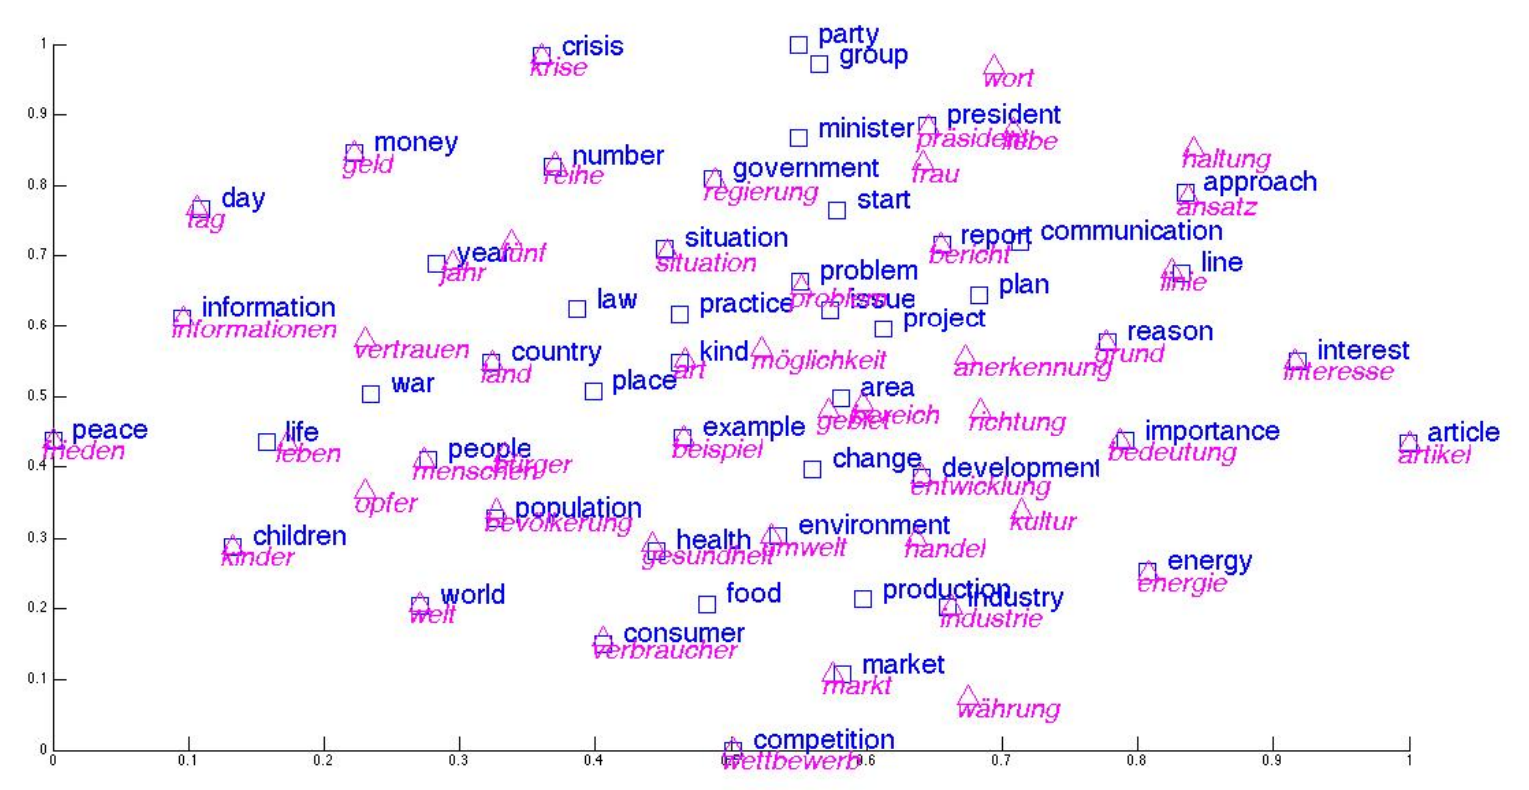
\includegraphics[width=14cm]{crossembedding}
		\centering
		\caption{A cross-lingual embedding space between German and English}
	\end{figure}
	
	In the thesis, I assume there are two set of embeddings ${e}$, ${f}$trained separately on monolingual data.  The propose of cross-lingual word embedding training is to learn such a mapping ${W \in }$ from source embedding space to target embedding space, so $Wf_i, e_j$ in the same embedding space and for all corresponding word pairs, we need to optimize the mapping ${W}$, so that" 
	\[ \arg\min_{W \in R^{d \times d}} \sum_{i} \lVert Wf_i - e_i \rVert \]
	where $d$ is the dimension of embeddings, and the distance ${\lVert Wf_i - e_i \rVert}$ can be different types. We prefer the Euclidean distance.  
	
	
	\subsection{Supervised Learning}
	According to the training method we can divide the supervised method into three:
	\begin{enumerate}
		\item Mapping based approaches\\
		First train the monolingual word embedding separately and then seek the seed dictionary to learn the mapping. 
		\item Pseudo-multi-lingual corpora-based approaches\\
		Use the monolingual embedding training method on constructed corpora that contains both the source and the target language.
		\item Joint methods\\
		Take the parallel text as input and minimize the source and target language losses jointly with the cross-lingual regularization term
	\end{enumerate}
	
	A dictionary is necessary for learning the cross-lingual word embedding. 
	minimizing the distance in a bilingual dictionary.\\
	
	Xing \cite{ } showed that the results are improved when we constrain the ${W}$ to be an orthogonal matrix. This constraint,  the optimal transformation can be efficiently calculated in linear time with respect to the vocabulary size.
	
	The problem then is simplified as the Procrustes problem and there exists a closed-form solution obtained from the SVD of ${EF^T}$
	
	\begin{figure}[t]
		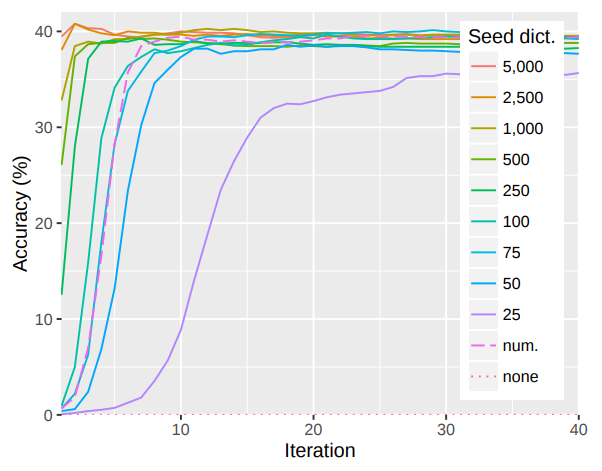
\includegraphics[width=12cm]{iter1}
		\centering
		\caption{Accuracy on bilingual lexicon induction}
	\end{figure}	
	
	\subsection{Unsupervised Learning}
	However, large dictionary is also not readily available for many language pairs.
	
	Several unsupervised learning algorithms are studies   
	
	Self-learning framework\\
	
	\begin{figure}[ht]
		\centering
		\begin{minipage}{.7\linewidth}
			\begin{algorithm}[H]
				\SetAlgoLined
				\KwIn{$\mathcal{F}$ (source embeddings)}
				\KwIn{$\mathcal{E}$ (target embeddings)}
				\KwIn{$\mathcal{D}$ (seed dictionary)}
				\KwResult{$\mathcal{W}$ (embedding mapping) }
				 \While{not converge}{
					 ${\mathcal{W} \leftarrow LEARN\_MAPPING(\mathcal{F},\mathcal{E},\mathcal{D})}$
					 ${\mathcal{D} \leftarrow LEARN\_DICTIONARY}$
										
				}
				
				\caption{Self-learning framework}
			\end{algorithm}
		\end{minipage}
	\end{figure}
	
	
	\begin{figure}[t]
		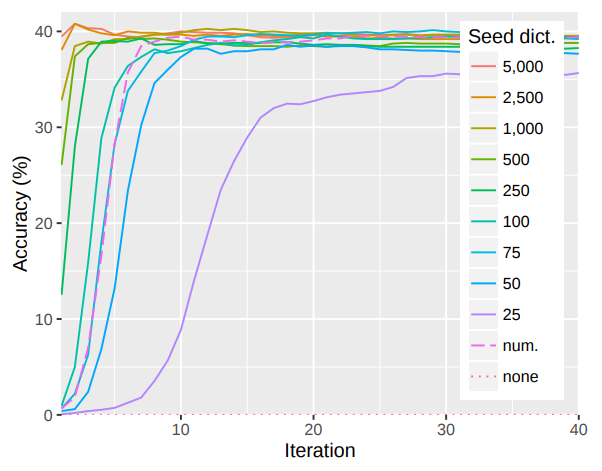
\includegraphics[width=12cm]{iter1}
		\centering
		\caption{Accuracy on bilingual lexicon induction}
	\end{figure}
	
	\cite{artetxe2018robust}.\\As it can be clearly observed that, the self learning algorithm can effectively learn the mapping between the source and target distribution even starts with a small dictionary size and the final accuracy when the algorithm converges are nearly the same level. However when start randomly without any support of dictionary, the framework does not work. In order to realize a fully unsupervised learning, we need to design heuristics to build the seed dictionary.
	
	\subsubsection{Unsupervised Initialization}
	For total unsupervised learning, there is no direct alignment between the languages. 	The most challenge for unsupervised learning is the initialization. As proved in the experiment of \cite{}, the self-learning framework can work even with a small dictionary set, however the model cannot work without such dictionary as hint.  So it is important to find heuristic methods to initialize the model.
	
	Several models are proposed:
	Based on matrices ${M_E = EE^T}$, ${M_F = FF^T}$, we can exploit latent information to reduce the mismatch. Assume that, the words in the source and target set are most common. For a specific word, the corresponding line in ${M_E}$ demonstrates the distribution of similarity in the source vocabulary. ${M_E}$, ${M_F}$ can be nearly equivalent up to a permutation of the words. 
	Instead of explore all the probability of permutation, he first sorts the values in each row of ${M_F}$ and ${M_E}$
	
	Assume the SVD of ${E = USV^T}$,  the similarity ${M_E = US^2U^T}$. In practice, he computed sorted ${1}$, ${2}$	yielding the matrix ${E^{\prime}}$ , ${F^{\prime}}$ and used to build the initial solution for self-learning.
	\subsubsection{Iterative Closest Point Method}
	Assume that many language pairs share same principle axes of variation. We do the approximate distribution alignment with PCA.
	For each language, we first select most frequent word vector,center the data and project it to the top ${p}$ principle components. We denote the projected language representation as 	${P_l \in {R}^{N * p}}$
	Propose a method first learn ${T_{ef}}$ and ${T_{fe}}$ for ${E \rightarrow F}$ and ${F \rightarrow E}$ , we include the cycle-constraints ensure that a word ${f}$ transformed into joint embedding space and transformed back is unchanged. 
	
	
	\begin{enumerate}
		\item For each ${e_i}$, find the nearest ${W_{fe} f_j}$.  denote as ${f(e_i)}$
		\item For each ${f_j}$, find the nearest ${W_{ef} e_i}$, denote as ${e(f_j)}$
		\item For all mini-barches of ${e_i}$ and ${f_j}$ in epoch, iterative optimize ${T_{ef}}$ and ${T_{fe}}$ on: \\
		${ \sum_{i} {\lVert e_i - W_{fe} f(e_i)\rVert} + \sum_j {\rVert f_j - W_{ef} e(f_j)\rVert} + \lambda {\sum_i}{\lVert e_i- W_{fe} W_{ef} e_i \rVert}  +  \lambda \sum_j {\lVert f_j - W_{ef} W_{fe} f_j \rVert}}$
	\end{enumerate}
	\subsubsection{Adversarial Training} 
	Discriminator is trained to discriminate between elements randomly sampled from ${Wf_i}$ and ${e_j}$ and generator ${W}$ is trained to prevent the discriminator from making accurate prediction\\
	
	The training algorithm follows the standard procedure of deep adversarial networks(GAN) of Goodfellow \cite{bibid}: the discriminator and generator are trained iteratively with the stochastic gradient descent to minimize the ${L_D}$ and ${L_w}$

	Let ${=\{ x_1, \cdots, x_n\}}$ and ${ = \{ y_i, \cdots , y_m\}}$ be the two sets of $n$ and $m$ word embeddings from a source and a target language separately, We refer the discriminator parameters as ${\theta_D}$.The discriminator is a multi-layer neural network trained to discriminate the transformed source word embedding from the target word embedding, while the mapping $W$, simply a linear transformation, is trained to fooling discriminator. In the two-player game, we are supposed to learn the mapping from source embedding space to the target space.
	Discriminator objective  
	\[ L_D(\theta_D | W) =  -\frac{1}{n} \sum_{i=1}^{n} \log P_{\theta_D}(source = 1| Wf_i) - \frac{1}{m} \sum_{i=1}^{m} \log P_{\theta_D}(source=0| e_i) \]	
	
	Mapping objective 
	\[ L_W(W|\theta_D) =  -\frac{1}{n} \sum_{i=1}^{n}\log P_{\theta_D}(source=0|W f_i) - \frac{1}{m} \sum_{i=1}^{m} \log P_{\theta_D}(source = 1 | e_i) \]
	
	
	\subsection{Cross-domain Similarity Local Scaling (CSLS)}
	The CSLS as described by \cite{conneau2017word}, can be written as:
	\[ CSLS(\bm{e}, \bm{f}) = 2 cos(\bm{e}, \bm{y}) - \frac{1}{K} \sum_{\bm{e^{\prime}} \in N(\bm{e})} cos(\bm{f}, \bm{e^{\prime}})- \frac{1}{K} \sum_{\bm{f^{\prime}} \in N(\bm{e})} cos(\bm{f^{\prime}}, \bm{e}) \]
	Since the embedding space is of high dimension and the nearest neighbour search is performed here, so that a few embeddings embedding will become the nearest neighbour of many data pointsto The obtained is known to suffer from the hubness problem, 
	We denote ${N_Y(x)}$ the set of ${K}$ nearest neighbors of points in the target embedding space, and ${N_X(y)}$ the nearest neighbors of ${y}$ in the source embedding space. 
	So in this way we penalize the hub points
	A good initialization is import for ICP methods, so begin with the projected data, and initialize transformation ${T_{ef}}$ and ${T_{fe}}$ with the identity matrix.
	After several iterations of, the estimated transformation becomes quite reliable.  Then use this transformation to find the matches.
	\subsubsection{Model Selection}
	Since the cross-lingual embedding training is under the unsupervised setting, We do not know the word translation accuracy, otherwise if we have the validation data, that means we will have parallel data, against the unsupervised idea. To address this issue, we must select from the property of data or the loss of the neural network as the unsupervised criterion. However in the experiments we find that the accuracy of the discriminator always stays at a high level no matter how is the word translation accuracy. 
	
	All these methods can be use to find meaningful word pairs in both languages. For further refinement we can use the induced dictionary to start the iterative self-learning algorithm. 
	
	